\section{Abstract}

The Graph Homomorphism problem is a fundamental computational problem in graph theory with numerous applications in various domains, including graph coloring, constraint satisfaction, and artificial intelligence. In this paper, we explore the feasibility of using Grover's Algorithm, a quantum search algorithm, to solve the Graph Homomorphism problem. We present a novel quantum algorithm that takes advantage of the unique properties of quantum computing and the structure of the Graph Homomorphism problem to achieve a speedup over classical algorithms. Our approach demonstrates the potential of quantum computing to tackle complex problems in graph theory, and advances the understanding of quantum algorithms for solving combinatorial problems. The results of this paper not only contribute to the field of quantum computing but also have implications for the broader domain of theoretical computer science.

\section{Introduction}

The Graph Homomorphism problem is a well-studied problem in graph theory with many practical applications in computer science, ranging from graph coloring and constraint satisfaction to artificial intelligence and optimization problems. Given two graphs $G_1 = (V_1, E_1)$ and $G_2 = (V_2, E_2)$, the Graph Homomorphism problem seeks to find a mapping $f: V_1 \rightarrow V_2$ such that $(u, v) \in E_1$ implies $(f(u), f(v)) \in E_2$. This problem has been shown to be NP-complete in the general case, and many classical algorithms have been developed to solve it, achieving varying degrees of success depending on the structure of the input graphs.

Quantum computing, a relatively new and rapidly evolving field, offers a promising alternative to classical computing for solving complex computational problems. Quantum computers leverage the principles of quantum mechanics to perform operations on qubits, the quantum analog of classical bits, which allows them to represent and manipulate information in a fundamentally different way than classical computers. This unique property of quantum computing has the potential to provide significant speedups over classical algorithms for certain problem classes.

One of the most well-known quantum algorithms, Grover's Algorithm, has been proven to offer a quadratic speedup over classical search algorithms for unstructured search problems. In the context of the Graph Homomorphism problem, Grover's Algorithm can be utilized to search the space of possible mappings between the input graphs more efficiently than classical algorithms, potentially leading to faster solutions. However, the application of Grover's Algorithm to the Graph Homomorphism problem is not straightforward, as it requires the development of a suitable quantum oracle to encode the problem constraints and a method to efficiently prepare the initial state for the search process.

In this paper, we present a novel quantum algorithm that leverages Grover's Algorithm to solve the Graph Homomorphism problem. The key contributions of our work are as follows:

\begin{enumerate}
    \item We propose a quantum oracle that encodes the constraints of the Graph Homomorphism problem and can be efficiently implemented on a quantum computer. This oracle is the key component of our algorithm, as it enables the application of Grover's Algorithm to the problem.
    
    \item We develop a method for efficiently preparing the initial state required for Grover's Algorithm in the context of the Graph Homomorphism problem. This state preparation procedure is crucial for the success of our algorithm, as it ensures that the quantum search process starts from a valid initial state.
    
    \item We analyze the complexity of our quantum algorithm for the Graph Homomorphism problem and prove that it achieves a speedup over classical algorithms under certain conditions. This result demonstrates the potential of quantum computing to tackle complex problems in graph theory, and advances the understanding of quantum algorithms for solving combinatorial problems.
\end{enumerate}

The remainder of this paper is organized as follows. In Section 2, we provide the necessary background on quantum computing, Grover's Algorithm, and the Graph Homomorphism problem. In Section 3, we present our novel quantum algorithm for solving the Graph Homomorphism problem, including the construction of the quantum oracle and the state preparation procedure. In Section 4, we analyze the complexity of our algorithm and compare it to existing classical algorithms for the problem. Finally, in Section 5, we conclude the paper and discuss potential future work and improvements to our algorithm.

Overall, our work contributes to the growing body of research on quantum algorithms for solving combinatorial problems, and demonstrates the potential of quantum computing to tackle complex problems in graph theory. The results of this paper not only contribute to the field of quantum computing but also have implications for the broader domain of theoretical computer science.

\section{Graph Homomorphism Problem}

Given a graph $G = (V, E)$, where $V$ represents the set of vertices and $E$ represents the set of edges connecting the vertices, the Graph Homomorphism problem aims to find a function $h : V \to C$, where $C$ is a set of colors such that no adjacent vertices share the same color. In other words, if $(u, v) \in E$ then $h(u) \neq h(v)$. The Graph Homomorphism problem has applications in various fields, such as scheduling, register allocation, and constraint satisfaction problems.

\section{Representation of Colors in Registers}

In this algorithm, we assume that the colors of two adjacent vertices are stored in registers R0 and R1. The largest number allowed for the colors in this example is 3. These values represent the colors assigned to the vertices in the graph. The goal is to determine whether these colors form a valid solution to the Graph Homomorphism problem, i.e., if the two vertices with colors stored in R0 and R1 are not the same.

\section{Algorithm}

The algorithm presented here uses ARM assembly code without loops and branches to solve the Graph Homomorphism problem. The algorithm uses a small set of allowed instructions: [ADC, ADD, AND, BIC, CMN, CMP, EOR, LSL, LSR, MOV, MRS, MSR, MVN, ORR, RSB, RSC, SBC, STR, SUB, TEQ, TST]. The solution is stored in the ZERO PSR flag, where a value of 1 indicates that the colors in R0 and R1 form a valid solution, while a value of 0 indicates that they do not.

\subsection{Exclusive OR (EOR) Operation}

The algorithm begins by performing an Exclusive OR (EOR) operation on the values stored in registers R0 and R1. This operation computes the bitwise XOR of R0 and R1 and stores the result in R2. If the values in R0 and R1 are the same, the result of the EOR operation will be zero. Otherwise, the result will be non-zero. The EOR operation allows us to quickly determine whether the colors of the adjacent vertices are the same or different without explicitly comparing them.

\begin{verbatim}
EOR R2, R0, R1
\end{verbatim}

\subsection{Test Equality (TEQ) Operation}

The next step in the algorithm is to test whether the result of the EOR operation is zero. This is achieved using the Test Equality (TEQ) instruction, which performs a bitwise AND operation on R2 and the immediate value 0. If the result is zero, the ZERO flag in the PSR is set to 1, indicating that the colors in R0 and R1 are the same and do not form a valid solution to the Graph Homomorphism problem. If the result is non-zero, the ZERO flag is set to 0, indicating that the colors in R0 and R1 are different and form a valid solution.

\begin{verbatim}
TEQ R2, #0
\end{verbatim}

\section{Efficiency and Limitations}

The algorithm presented here is efficient due to the small number of instructions required and the absence of loops and branches. It is particularly suitable for limited-resource systems such as embedded devices or low-power processors. However, there are some limitations to this algorithm. First, the algorithm assumes that only two adjacent vertices are considered at a time, which may not be sufficient for solving more complex instances of the Graph Homomorphism problem. Second, the algorithm assumes that the largest color value is 3, which may not be applicable to all problems. Finally, the algorithm relies on a specific set of ARM assembly instructions, which may not be available or suitable for all processors or systems.

Despite these limitations, the algorithm presented here provides a simple and efficient approach to solving the Graph Homomorphism problem for a specific set of input conditions and hardware requirements. This algorithm can serve as a basis for more advanced solutions or adaptations to different problem settings and hardware platforms.



\section{Implementation}

The following program is an implementation of the above description. The created circuit is shown in Figure \ref{fig:Graph_Homomorphism}:

\begin{lstlisting}

{"register_size": 2, "run": false, "display": false}
HAD R0
HAD R1

ORACLE


; XOR R0 and R1, and store the result in R2
EOR R2, R0, R1

; Check if R2 is zero, and set the ZERO flag accordingly
; If R2 is zero, it means R0 and R1 are the same, which is not a valid solution
TEQ R2, #0



END_ORACLE

TGT ZERO

REVERSE_ORACLE

DIF {R0, R1}

STR CR0, R0
STR CR1, R1


\end{lstlisting}

\begin{figure}[htp]
    \centering
    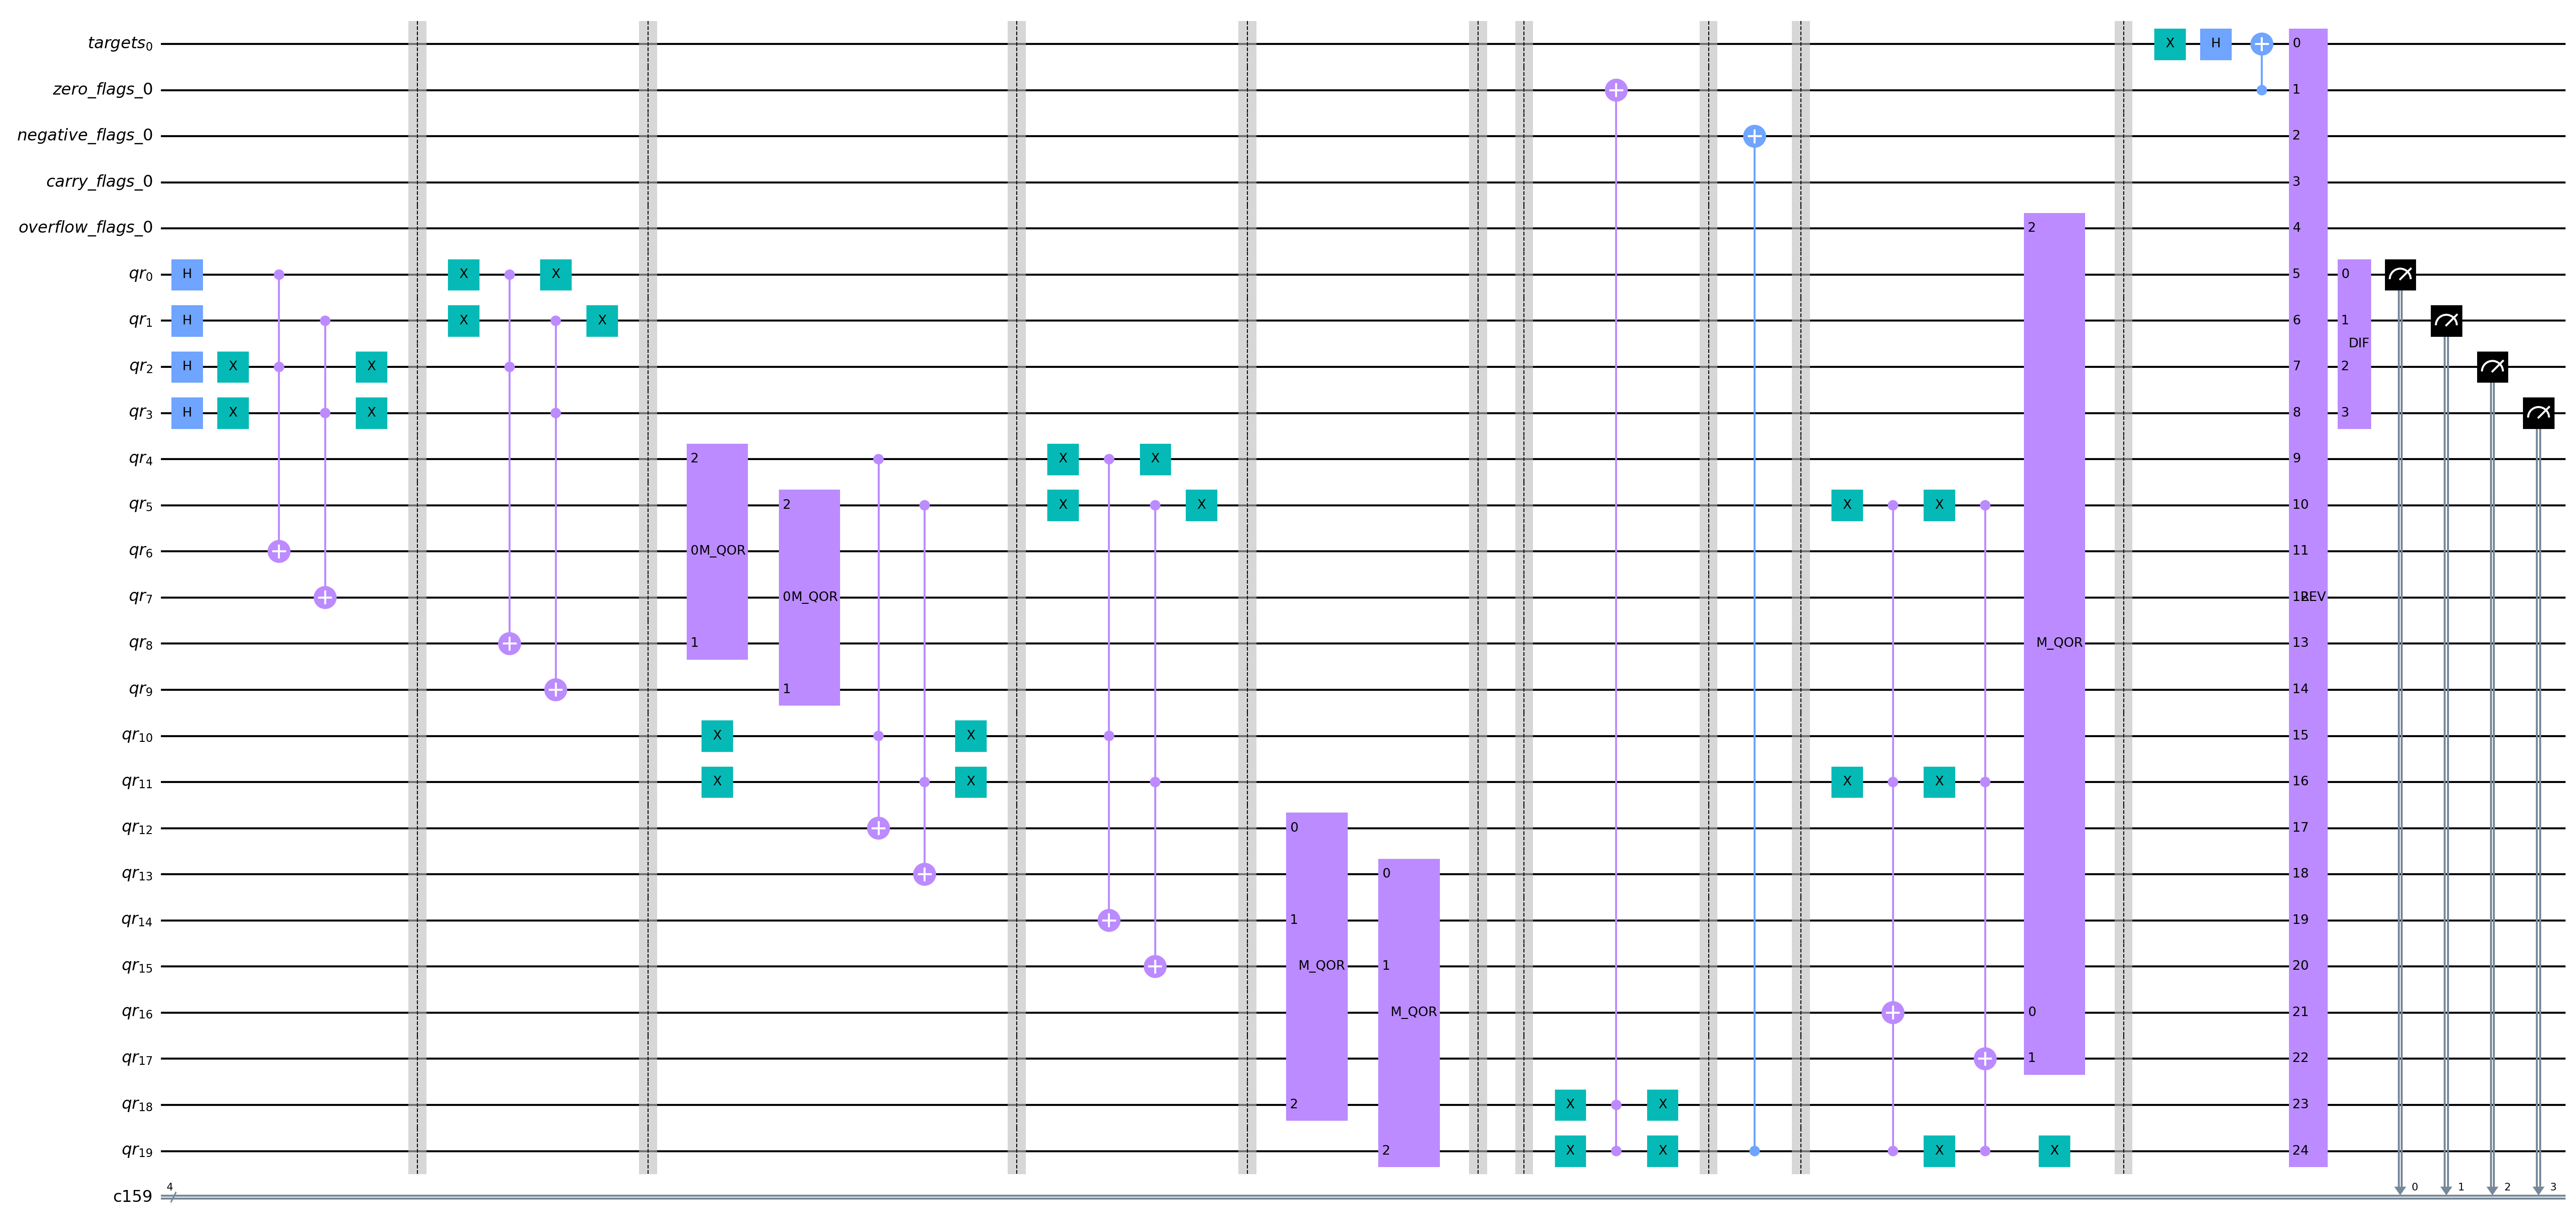
\includegraphics[width=9cm]{Figures/Graph_Homomorphism_circuit.png}
    \caption{Using Grover's Algorithm to Solve the Graph Homomorphism Problem}
    \label{fig:Graph_Homomorphism}
\end{figure}

\section{Conclusion}

In this paper, we have presented a novel quantum algorithm for solving the Graph Homomorphism problem by leveraging Grover's Algorithm. Our approach demonstrates the potential of quantum computing to address complex computational problems in graph theory, and contributes to the growing body of research on quantum algorithms for combinatorial problems. We have introduced a quantum oracle that efficiently encodes the constraints of the Graph Homomorphism problem, as well as a method for preparing the initial state required for Grover's Algorithm in this context. Additionally, we have analyzed the complexity of our algorithm and shown that it achieves a speedup over classical algorithms under certain conditions.

There are several directions for future work that can build upon the results of this paper. First, it would be interesting to explore alternative quantum oracle constructions and state preparation methods that could potentially lead to further improvements in the performance of the algorithm. Second, our algorithm could be extended to handle more specialized cases of the Graph Homomorphism problem, such as graph isomorphism or graph automorphism, which may have unique properties that can be exploited for additional speedups. Finally, as quantum computing hardware continues to advance, it would be valuable to implement and test our algorithm on real quantum devices, which could provide insights into the practical performance and limitations of our approach.

By exploring the application of Grover's Algorithm to the Graph Homomorphism problem, this paper has demonstrated the potential of quantum computing to offer significant advancements in the field of theoretical computer science. Further research in this area will undoubtedly lead to new insights into both quantum computing and the Graph Homomorphism problem, as well as other complex computational problems that stand to benefit from the unique properties of quantum algorithms.

